%!TEX root = ../document.tex
\chapter{Grundlagen} \label{chp:Grundlagen}  
In den folgenden Abschnitten werden eine Reihe von Begriffen und Verfahren genutzt, die hier eingeführt werden sollen.     
Dies ermöglicht dem Leser die Beantwortung der Fragestellungen aus Abschnitt \ref{chp:Loesungsansatz} nachzuvollziehen.    
 
Zunächst werden einige geografische Grundbegriffe eingeführt. 
Danach wird auf Twitter eingegangen, es werden grundsätzliche Funktionen und Begriffe von Twitter eingeführt. 

 
Zum Schluss wird die genutzte Datenbasis und der Einfluss der von Twitter genutzten Sampling-Strategie vorgestellt und erläutert.

\newpage

	\section{Geografische Grundlagen und Begriffe}
	In diesem Kapitel sollen geografische Grundbegiffe erläutert werden. 
	Einige geografische Begriffe werden in verschiedenen wissenschaftlichen Bereichen unterschiedlich genutzt und teilweise widersprüchlich definiert. 
	Um Missverständnissen vorzubeugen wird hier definiert was in der vorliegenden Arbeit unter den einzelnen Begriffen zu verstehen ist.
	Eine Reihe von Begriffen wird selbst definiert um bestimmte Sachverhalte im Kontext dieser Arbeit klarer ausdrücken zu können. 

		\paragraph*{Geodätisches Referenzsystem} 
		Ein geodätisches Referenzsystem dient als einheitliche Grundlage zur Angabe einer Position auf der Erde. 
		In diesem Referenzsystem werden unter anderem Referenzpunkte und ein geeignetes Koordinatensystem festgelegt. \footnote{Vergleiche Geoinformatik Lexikon der Universität Roctock: http://www.geoinformatik.uni-rostock.de/lexikon.asp und Vorlesungen zur Geo-Informatik von Prof. Dr.-Ing. Ralf Bill : http://www.geoinformatik.uni-rostock.de/vorlesungsthem.asp \label{ft:geoinfolex} }   
		
		\paragraph{Georeferenz}
		Eine Georeferenz (engl. Spatial Reference) wird auch als Raumbezug bezeichnet. 
		Unter dem Begriff der Georeferenz versteht man die zugeordnete der Lage beziehungsweise Position zu einem Datensatz. 
		Die konkreten Angaben zum Raumbezug und deren Genauigkeit hängen von den Anforderungen ab, die an die Georeferenz gestellt wird. 
		Auch die in Kapitel \ref{chp:Einleitung} erwähnten Anwendungen stellen unterschiedliche Anforderungen an die Genauigkeit der Georeferenz.
		Die Georeferenz lässt sich weiter unterteilen in: 
		\footref{ft:geoinfolex} 
		
			\begin{description}
	 			\item[Direkte Georeferenz (direkter Raumbezug)] 
	 			Unter direktem Raumbezug versteht man die Angabe einer konkreten Koordinate bezüglich eines geeigneten, unveränderlichen geodätischen Referenzsystems. 
	 			\item[Indirekte Georeferenz (indirekter Raumbezug) ] 
	 			Unter indirektem Raumbezug werden alle Angaben verstanden die eine ungenaue Position bezüglich eines beliebigen Referenzysystems bestimmen.
	 			Ungenau ist in dem Sinne zu verstehen, dass die Angabe der Position auch eine Fläche beschreiben kann.
	 			Zusätzlich muss das gewählte Referenzsystem nicht zwingenderweise unveränderlich sein.   
	 			Beispiele für die Angabe eines indirekten Raumbezugs wären Länder, Adressen, Postleitzahlen oder auch Telefonvorwahlen. 
	 			Alle diese Angaben, mit Ausnahme der Adresse, definieren eine geografische Fläche. 
	 			Diese Fläche ist nicht zwingenderweise klar abzugrenzen.
			\end{description}

		\paragraph{geografische Objekt}
		Ein geografisches Objekt, ist ein Objekt der Realwelt, dessen Position durch eine Georeferenz bestimmt werden kann. 
		Die EN ISO 19110 Norm beschreibt ein geografisches Objekt folgendermaßen:
		"'Geographische Objekte sind Erscheinungen der realen Welt, die einen Bezug zur Erde (Raumbezug) haben..."'

		\paragraph*{Toponyme}
		Ein Toponym ist ein konkreter Name für ein geografisches Objekts. 
		Beispiele hierfür sind: Städtenamen, Ländernamen oder Landschaftsnamen.  

	 	\paragraph*{Georeferenzierung}
		Unter Georeferenzierung versteht man die Zuordnung einer Georeferenz zu einem Datensatz. 
		Also den Vorgang einem Datensatz, zum Beispiel einem Twitter-Nutzer eine Georeferenz zuzuordnen. \footref{ft:geoinfolex} 

	 	Aufrgund der einfacheren Verständlichkeit werden die folgenden zwei Begriffe definiert, welche in der restlichen Arbeit verwendet werden.

		\paragraph*{Geografische Position}
		Unter geografischer Position wird hier ein konkreter Ort, unter Angabe geografischer Koordinaten verstanden.
		Eine geografische Position entspricht somit einer direkten Georeferenz (direktem Raumbezug).

		\paragraph*{Geografische Region} 
		Unter einer geografischen Region werden Flächen verstanden welche nicht mit einem Punkt, in Form von Längen- und Breitengrad, beschrieben werden können. 
		Hierbei kann es sich beispielsweise um Bundesländer oder Länder.
		Somit entspricht der Begriff geografische Region einer indirekten Georeferenz (indirektem Raumbezug).

		\paragraph*{Geografische Hierarchie} \label{par: geografische Hierarchie} 
		In der vorliegenden Arbeit wird eine geografische Hierarchie verwendet um eine Einteilung der Erde in geografische Regionen umzusetzen.
		Dabei können geografische Regionen wiederum geografische Regionen oder geografische Positionen enthalten, wodurch sich eine hierarchische Gliederung ergibt.
		Diese Einteilung spiegelt im wesentlichen die Einteilung der Erde in Staaten und deren individuellen Verwaltungseinheiten wieder.
		Im vorliegenden Fall ist das Staatsgebiet, also die Fläche über die sich der Staat erstreckt, von Interesse. \footnote{Zur genauen Definition eines Staatsgebietes vergleiche \cite{jellinek1921}} 

		Im Gegensatz dazu könnte die Erde auch in ein Gitternetz eingeteilt werden. 
		Die einzelnen Zellen würden dann als Referenz für eine geografische Region verwendet werden.
		Dieses vorgehen wird unter anderem in \cite{Serdyukov2009} angewendet.

		Eine Aufteilung der Erde in geografische Regionen lässt sich auf oberster Ebene mit Hilfe von Ländern und deren Grenzen umsetzen. 
		Daraus resultiert eine Einteilung, welche direkt intuitiv verständlich ist und vielen Anforderungen an geografische Informationen gerecht wird.
		Die meisten Länder sind in weitere administrative Einheiten aufgeteilt.
		Diese geografischen Regionen werden hier als Administartionsebenen bezeichnet.
		Es wird zwischen Administrationsebenen erster und zweiter Ordnung unterschieden. 
		Ausnahmen sind besipielsweise Stadtstaaten wie der Vatikan-Staat oder das Fürstentum Monaco, welche aufgrund ihrer Größe nicht in Verwaltungsbezirke unterteilt werden und keine Städte.
		Des weiteren werden in der untersten Ebene der Hierarchie Städte dargestellt.

		Wenn man als Beispiel Deutschland heranzieht, ergibt sich eine Einteilung wie in Bild \ref{img:hierarchy} dargestellt wird. \footnote{Aus Platzgründen sind im Bild pro Ebene nur einige wenige geografische Objekte aufgezählt.} 
		Die oberste Ebene beschreibt das Land worauf die zweite Ebene die Bundesländer darstellt.
		Auf der dritten Ebene werden die Regierungsbezirke abgebildet, worauf die Städte in der letzten Ebene folgen. 
		Analog kann die Einteilung für die USA vorgenommen werden, woraus sich die Hierarchie Country->State->County->City ergibt.

		Bis auf die letzte Ebene wird den Objekten in der Hierarchie eine geografische Region zugeordnet. 
		Lediglich die unterste Ebene, die der Städte, wird durch eine geografische Position exakt beschrieben. 
		Die Ausdehnung einer Stadt wird in der gegebenen Hierarchie also nicht berücksichtigt. 
		Jede Stadt wird als konkrete geografische Position mit Koordinaten repräsentiert. 

		\begin{figure}[h!]
		\begin{center}
		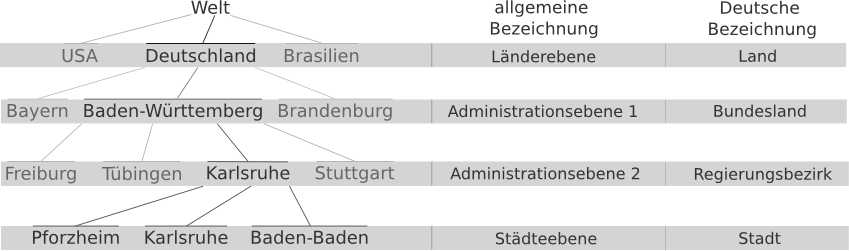
\includegraphics[scale=0.5]{hierarchie.png}
		\caption{Die Hierarchiebenen exemplarisch. Bis in die Städtebene wird nur der Pfad Welt -> Deutschland -> Baden-Württemberg -> Karlsruhe ->K arlsruhe,Pforzheim,Baden-Baden dargestellt.}
		\label{img:hierarchy}
		\end{center}
		\end{figure}	

		\paragraph*{Ortsverezichnis}
		Oder auch Gazetteer genannt. Auch auf Geocoding API eingehen. 	  




	\section{Twitter} 
	In diesem Kapitel werden grundlegende Begriffe rund um das Twitter-Netzwerk erläutert. 
	Weiter werden die Mechanismen in Twitter erläutert und an praktischen Beispielen erklärt. 
	Zum Schluss wird aufgezeigt welche Informationen pro Tweet übermittelt werden und welche Daten zur Lokalisierung verwendet werden können.

		\subsection{Geschichtliches}
		Twitter wurde 2006 von Jack Dorsey, Biz Stone, Noah Glass und Evan Williams gegründet.
		Ursprünglich war Twitter zur internen Kommunikation innerhalb der Firma Odeo geplant.
		Schnell wurde allerdings klar, dass in dem Dienst mehr potenzial steckt und so wurde Twitter öffentlich gemacht.
		Seitdem erfreut sich der Dienst einer wachsenden Nutzer-Gemeinde.
		Die Twitter-Gründer haben von Anfang an keine exakten Nutzer-Zahlen oder die Anzahl der versendeten Twitter-Kurznachrichten bekanntgegeben.
		Dies geschah einerseits, weil die Gründer davon überzeugt sind, dass anhand der reinen Nutzer-Zahlen und gesendeten Twitter-Kurznachrichten nicht die '"Gesundheit"' des Twitter-Netzwerks nachvollzogen werden kann, andererseits werden durch diese Massnahme auch strategische Ziele verfolgt.  \footnote{http://www.pbs.org/mediashift/2007/05/twitter-founders-thrive-on-micro-blogging-constraints137}
		2013 ging Twitter an die Börse und vermeldete 100 Millionen täglich aktive Nutzer und über 500 Millionen Twitter-Kurznachrichten, die täglich über den Dienst versendet werden. 

		\subsection{Was ist Twitter?}
		Twitter wird als Kurznachrichten-Dienst, Mikroblogging-Dienst oder auch als soziales-Netzwerk bezeichnet. 
		Twitter Geschäftsführer Kevin Thau hat 2010 auf dem Nokia-World Kongress öffentlich bestritten, dass Twitter ein Soziales-Netzwerk ist. 
		Laut Thau handelt es sich um ein Nachrichten-, Inhalts- und Informations-Netzwerk. 
		Er begründete dies damit, dass Twitter die Art und Weise wie Nachrichten verteilt werden geändert hat und praktisch jeder zum Journalisten werden kann. 
		Als Beispiel nennt er die Landung des Fluges 1549 auf dem Hudson River. 
		Die Augenzeugen hätten damals keine Mails versendet um die Nachricht zu verbreiten, sondern die Nachricht via Twitter weitergegeben.
		Es lassen sich eine Reihe weitere Beispiele derselben Art finden. 
		In \cite{Petrovic2013} wird ein Vergleich zwischen sogenannten Newswire anbietern und Twitter gezogen. \footnote{Newswire stellt eine Art Nachrichtenaggregator dar, über welchen Nachrichten aus verscheidenen Quellen aggregiert und weitergegeben werden. In deutschland kommt die Deutsche Presse agentur diesem Konzept am nächsten.}
		Es stellte sich heraus, dass über nahezu alle Nachrichten, welche in den Newswires verbreitet wurden auch im Twitter-Netzwerk berichtet wird.
		Nachrichten zu bestimmten, vermutlich sehr speziellen Themen oder Auslandsnachrichten wurden ausschliesslich in Twitter gefunden. 
		Diese Erkenntnisse decken sich mit der Einschätzung von Kevin Thau. 
		In \cite{Kwak2010} wird die Einschätzung, bei Twitter handele es sich nicht um ein soziales Netzwerk, wissenschaftlich bestätigt.
		Kwak et al überprüfen die in \cite{Newman2003} beschriebenen Eigenschaften sozialer Netzwerke und kommen zu dem Schluss, dass Twitter diese Eigenschaften nicht erfüllt.	

		Die Bezeichnung Kurznachrichten-Dienst ist irreführend, da dieser mit sms (small messeneger service) in Verbindung gebracht werden kann. 
		Tatsächlich galt der sms in der Anfangsphase von Twitter als Vorbild für den Dienst.
		In Twitter werden Nachrichten allerdings standardmäßig allen Benutzern zur Verfügung gestellt und können eingesehen werden. 
		Des weiteren wird eine Liste der Nachrichten, welche von einem Nutzer verfasst wurden, als Liste in umgekehrter chronologischer Reihenfolge auf dessen Profil dargestellt.
		Damit ähnelt das Twitter-Profil einem Blog mit Einträgen deren Länge 140 Zeichen nicht überschreiten darf. 
		Die Darstellung als Liste, und die Funktion einen Tweet standardmäßig allen Nutzern freizugeben unterscheidet sich grundlegend von der Funktion des sms, bei dem eine Nachricht direkt an einen Empfänger gesendet wird und nicht öffentlich ist.
		Im sms steht die Konversation zweier Nutzer im Vordergrund, wohingegen Nachrichten im Twitter-Netzwerk einen Brodcast an alle Nutzer darstellen.

		Die 140 Zeichen langen Nachrichten in Twitter werden als Tweets bezeichnet.
		Tweet bedeutet übersetzt Zwitschern, womit die Redenwendung '"Die Spatzen zwitschern es von den Dächern"' auch im Twitter-Netzwerk zu einer passenden Redenwendung  wird.  
		In der vorliegenden Arbeit wird Twitter deshalb als Mikroblogging-Dienst bezeichnet.
	

		\subsection{Funktionen von Twitter}
		Der Mikroblogging-Dienst Twitter bietet neben dem Profil, auf dem die Tweets des Nutzers angezeigt werden, noch eine Reihe weiterer Funktionen. 
		Im folgenden soll das Twitter-Profil und die Timeline kurz erläutert werden. 
		Eine der zentralen Funktionen von Twitter ist das sogennante Folgen, womit sich Nutzer win Netzwerk aufbauen können aus dem sie Twitter Nachrichten erhalten.
		Danach werden Funktionen wie das weitergeben eines Tweets, Favorisieren und Antworten erklärt. 
		Zum Schluss wird auf den gesendeten Tweet Inhalt eingenagen und der Netzwerk-Charakter von Twitter untersucht.

		\begin{figure}[h!]
		\begin{center}
		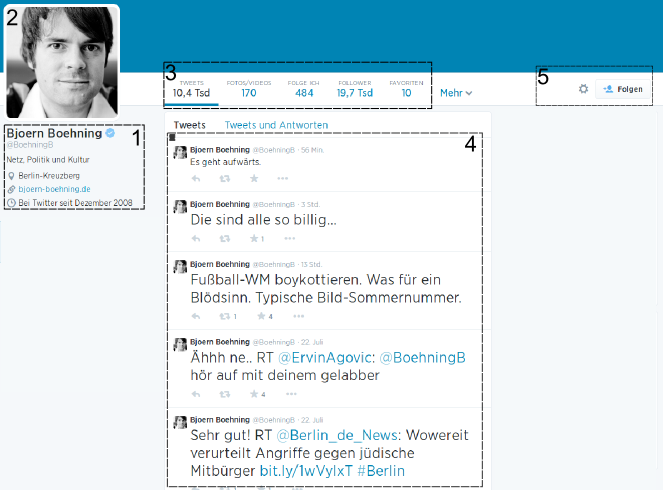
\includegraphics[scale=0.4]{profile.png}
		\caption{Die Twitter-Timeline auf einem Twitter Profil. 1: Nutzername und Informationen über den Nutzer. 2: Profilbild
		3: Allgemeine Informationen über den Benutzer und dessen Netzwerk
		4: Nutzer-Timeline: Tweets des Nutzer in umgekehrter chronologischer Reihenfolge 
		5: Button zum Folgen}
		\label{img:twitterProfile}
		\end{center}
		\end{figure}	


			\paragraph{Das Nutzer-Profil und die Nutzer-Timeline}
				Das Nutzer-Profil kann über die Url http://twitter.com/BENUTZERNAME abgerufen werden und bietet neben der Nutzer-Timeline, in der die Tweets des Nutzers angezeigt werden, eine Reihe an weiteren Informationen.
				In Abbildung \ref{img:twitterProfile} ist in der mitte die Timeline des Benutzers dargestellt in der dei Tweets zu sehen sind. 
				Unter dem Profilbild links sind Informationen des Nutzers aufgelistet.
				Diese Informationen kann der Nutzer selbst einstellen und entscheiden welche er angeben möchte.   


			\paragraph{Folgen (Following/Follower/Tweeps)}
				Diese Funktion erlaubt es Tweets eines bestimmten Nutzers zu abonnieren. 
				Im Twitter-Umfeld spricht man von '"following"' oder '"folgen"', wenn man die Tweets eines bestimmten Nutzers abonniert.
				Hat man Tweets eines bestimmten Nutzers abonniert so wird man als dessen '"Follower"' bezeichnet. 
				Das englische Wort '"Follower"' hat sich im Twitter-Umfeld und darüber hinaus eingebürgert und wird selten übersetzt. 
				Auch auf der Twitter Website wird '"Follower"' nicht ins deutsche übersetzt.
				In der vorliegenden Arbeit wird deshalb auch auf eine Übersetzung verzichtet. 

				In Abbildung \ref{img:twitterProfile} an Position 3 wird unter '"Folge ich"' die Anzahl der Twitter-Nutzer angezeigt denen der Beispielnutzer folgt. 
				Neben dem Feld '"Folge ich"' wird unter '"Follower"' angezeigt wieviele Nutzer dem Beispielnutzer folgen.

			\paragraph{Persönliche Timeline}
				Jeder Twitter-Nutzer hat seine persönliche Timeline, auf dieser werden die Tweets derjenigen Nutzer angezeigt, denen er folgt. 
				Die Timeline kann als Aggregation von Tweets betrachtet werden.
				Diese Timeline ist die zentrale Stelle, an der die Nutzer Tweets anderer Nutzer empfangen und lesen.
				Auch hier werden die Tweets in umgekehrter chronologischer Reihenfolge angezeigt.  

			\paragraph{Weiterleiten eines Tweets (Retweet)}
				Unter einem Retweet versteht man das weiterleiten eines Tweets den man nicht selbst verfasst hat an die eigenen Follower.
				Genauer gesagt wird der Tweet übernommen und ein Hinweis hinzugefügt, dass es sich um einen sogenannten Retweet handelt, und nicht einen vom Nutzer selbst verfassten Tweet.
				Diese Funktion wird hauptsächlich genutzt um Nachrichten schnell zu verbreiten ohne diese neu eingeben zu müssen. 
				Die Weitergabe an die eigenen Follower impliziert einen gewissen Grad an Kontrolle und Filterfunktion. 
				Der weitergebende Nutzer kontrolliert und filtert die Nachrichten die er erhält und gibt diejenigen weiter, denen er eine Gewisse Relevanz beimisst, oder von denen er erwartet, dass sie seine Follower interessieren. \todo{1 retweet Reichweite 1000 Nutzer}
				Mit dieser Funktion können einzelne Nutzer eine Art Filterfunktion übernehmen, welche früher Journalisten vorbehalten war. 
				Es darf jedoch nicht vergessen werden, dass der Nutzer nur im Rahmen seiner eigenen Möglichkeiten einen Tweet verifizieren kann und Nachrichten in Twitter keinesfalls gesicherte Fakten darstellen.
				Auch können Nutzer durch diese Funktion zu Tweet-Aggregatoren werden, welche Tweets von mehreren Nutzern erhalten oder sammeln, aber nur relevante oder themenspezifische Tweets weitergeben.

				\todo{Diagramm Retweet, Filterfunktion} 

			\paragraph{Hashtags}
				Hashtags werden genutzt um Tweet Nachrichten zu kategorisieren oder Metag Informationen zu liefern. 
				Ein Hashtag kann vom verfasser selbst als solches ausgezeichnet werden indem ein \# vor das gewünschte Wort, welches als Hashtag fungieren soll, gesetzt wird. 
				Hahstags ermöglichen es Tweets nach Stichworten zu filtern. 
				Anhand der Hashtags werden auch die Twitter-Trends analysiert.
				Twitter Trends 
				
			\paragraph{Antworten und direktes ansprechen eines Nutzers}
				Twitter bietet die Möglichkeit einzelne Nutzer direkt anzusprechen. 
				Mit Hilfe des @-Symbols kann ein Nutzer referenziert werden. 
				Der referenzierte Nutzer, besipielsweise @alfred, wird dann benachrichtigt, dass er in einem Tweet erwähnt wurde. 
				Der erwähnte Nutzer muss dabei nicht Follower des Verfassers sein. \todo{siehe Bild ref1} 
				Eine weitere Funktion im Twitter-Netzwerk ist das Antworten auf einen Tweet.
				Über eine Schaltfläche wird es ermöglicht auf einen Tweet zu Antworten. 
				Das @-Symbol und der Nutzername des Verfassers werden automatisch eingetragen, womit eine Benachrichtigung an den Verfasser des Ursprungstweets erfolgt. \todo{siehe Bild ref2}
				Es ist möglich, das auf einen Antwort-Tweet wiederum geantwortet wird, wodurch ein sogenannter Thread oder Konversation entsteht. \todo{siehe Bild ref3}
				Auch ist es möglich, dass an einer solchen Konversation mehrere Twitter-Nutzer beteiligt sind. 
				Dies ist dann der Fall, wenn im ursprünglichen Tweet, auf weitere User referenziert wurde. 
				Aber auch wenn ein Nutzer auf eine bestehende Konversation antwortet, werden alle beteiligtien Nutzer referenziert. \todo{siehe Bild ref4}
				\todo{Diagramm Antwort, Antwort Thread, Bild Antworten Button, Referenzieren}     


			\paragraph{Favorisieren}
				Mit dieser Funktion lässt sich ausdrücken, dass man einen Tweet interessant oder gut findet.
				Auch Zustimmung wird durch favorisieren ausgedrückt.  
				Einen Tweet zu favorisieren kann aber auch bedeuten '"ich habe deine Reaktion registriert"', oft um einen Antwort-Thread nicht abrupt abzubrechen sondern eine zustimmende Rückmeldung zu geben ohne extra einen Tweet zu verfassen.

		\subsection{Daten einer Twitter-Nachricht}
			Neben den direkt sichtbaren Informationen enthält ein Tweet eine Reihe weiterer Daten.
			Betrachtet man einen einzelnen Tweet, beispielsweise auf twitter.com, wird der Tweet-Text, der Verfasser und die Zeit, wann der Tweet verfasst wurde, mitgeteilt. \todo{siehe Bild} 
			Die Gesamtheit der Daten die in einem Tweet enthalten sind werden hier allgemein als Tweet-Daten bezeichnet.

			\begin{figure}[h!]
			\begin{center}
			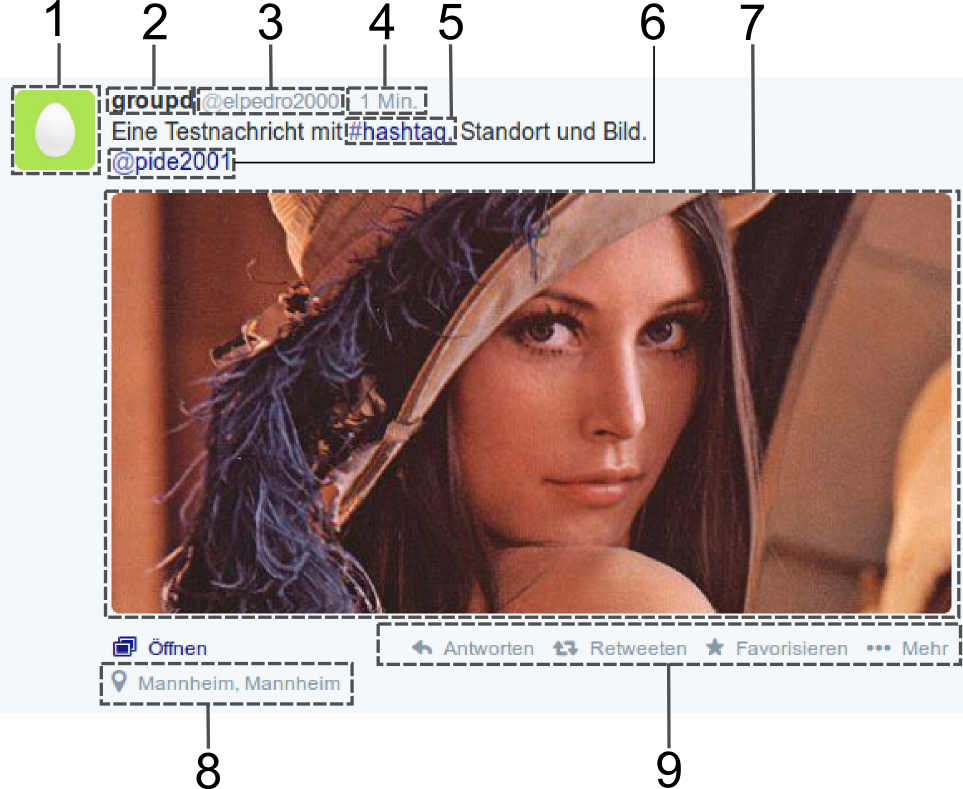
\includegraphics[scale=0.8]{tweetFinal.png}
			\caption{Was ist zu sehen?}
			\label{tweet}
			\end{center}
			\end{figure}	


			\paragraph{Koordinaten}
				In den Tweet-Daten können geografische Koordinaten in Form von Längen- und Breitengrad angegeben sein. 
				Diese Koordinaten zeigen an wo sich der Verfasser befand als er den Tweet abgesetzt hat.
				Wenn diese Koordinaten angegeben sind hat der Nutzer explizit zugestimmt, dass die Koordinaten seines aktuellen Aufenthaltsortes dem Tweet angehängt werden. 
				Die Bestimmung der Koordinaten und das anhängen der Koordinaten an einen Tweet werden vollautomatisch durch das Programm übernommen mit welchem der Tweet verfasst wurde.
				Auf Smartphones wird meist das integrierte GPS-Modul genutzt um die Koordinaten zu bestimmen. 
				Bei der Nutzung an einem PC wird der Tweet häufig über den Browser verfasst und die Position mit Hilfe von GeoIp ermittelt.





		 	\paragraph{Daten}
		 		Neben den sichtbaren Daten, welche in der Timeline angezeigt werden, enthält ein Tweet eine Reihe weiterer interessanter Informationen. 	


		 \subsection{geografischer Indikator}
		
			Unter einem geografischen Indikator wird eine Angabe verstanden, welche direkt einem Nutzer zugeordnet werden kann und die Auskunft über die geografische Position oder Region des Nutzers geben kann.
			Im Zuge dieser Arbeit wurden potentielle geografische Indikatoren untersucht und eine Reihe von Eigenschaften identifiziert anhand derer sich geografische Indikatoren kategorisieren lassen. 
			Diese Eigenschaften haben Einfluss darauf, wie und ob eine Georeferenz aus dem Indikator abgeleitet werden kann.
			Dabei ist zu unterscheiden ob sich die Eigenschaft auf den, durch den Nutzer eingegebenen, Wert bezieht oder auf die Information die durch die Angabe geliefert werden soll. 

			\subsubsection{Objektivität der Werte geografischer Indikatoren} 
				
				Der Wert eines geografischen Indikators ist genau dann objektiv wenn zwei Nutzer für denselben geografischen Ort oder dieselbe geografische Region immer den selben Wert eingeben.
				Ein Beispiel für einen objektiven geografischen Indikator wäre eine Liste von Ländern aus der ein Nutzer wählen kann.
				Der Nutzer hat dabei eine Wahl, kann aber nur aus einem begrenzten Anzahl an Möglichkeiten wählen. 

				Geben zwei Nutzer unterschiedliche Werte ein, obwohl sie denselben Ort oder dieselbe Region beschreiben wollen, ist dieser Wert nicht objektiv.

			\subsubsection{Zuverlässigkeit der Werte geografischer Indikatoren}
				
				Ein Wert ist genau dann zuverlässig wenn er in jedem Fall die Information enthält, welche durch das Feld repräsentiert werden soll. 
				Unzuverlässig ist der Wert, wenn er nicht in jedem Fall die Information enthält welche druch das Feld repräsentiert werden soll.  

			\subsubsection{Gesicherte Werte geografischer Indikatoren} 
				
				Als gesichert gilt ein Wert genau dann wenn die enthaltene Information in jedem Fall dem tatsächlichen Wert entspricht. 
				Im Umfeld von Twitter ist diese Eigenschaft nicht stichhaltig nachzuprüfen. 
				Alle Angaben die ein Benutzer eingibt werden nicht verfiiziert und können dementsprechen auch nicht gesichert sein. 
				Es besteht die Möglichkeit das ein Nutzer in jedem Feld Falschangaben macht. 
				Dies gilt es im erarbeiteten Verfahren zu beachten.


			\subsubsection{mittelbare und unmittelbare geografische Indikatoren}
				
				Diese Eigenschaft bezieht sich, im Gegensatz zu den vorgenannten auf die Information die durch das Feld oder die Eingabe repräsentiert werden soll. 
				
				Hierbei handelt es sich um Indikatoren welche unter Umständen einen geogarfischen Bezug haben können, aber die Intention bei der Eingabe war nicht eine geografische Position mitzuteilen.

				Beispielsweise die Verwendung bestimmter umgangssprachlicher oder dialektischer Wörter die einen Hinweis auf eine geografische Region geben können.
				Die Intention des Nutzers war nicht, dadurch einen Hinweis auf die geografische Position oder seinen Aufenthalstort zu geben, allerdings lässt sich mittelbar eine geografische Region daraus ableiten. 

			\subsubsection{unmittelbare geografische Indikatoren in Tweet-Daten}
				
				Unmittelbare geografische Indikatoren sind solche aus denen direkt eine geografische Position abgeleitet werden kann.

				 bzw. die Intention des Nutzers bei der Eingabe darauf abzielt eine geografische Position zu beschreiben.  
				Mit einer Gewissen Sicherheit kann ein geografischer Bezug abgeleitet werden, da die Intention des Feldes einen Standort angibt. 




	 	\subsection{Geoinformationen in Twitter Daten}
	 		\todo{Überarbeiten subsec:Geoninformationen in Twitter Daten} 
	 		\subsubsection{Welche Tweet-Daten können zur Georeferenzierung herangezogen werden} \todo{Nur optional} 

				Um diese Frage zu beantworten, müssen die Tweet-Daten eingehend untersucht werden. 
				Dabei spielt nicht nur die reine Information die den Daten entnommen werden kann eine Rolle, sondern auch wie die Daten generietr oder eingegeben wurden.
				Beispielsweise kann bei einem Tweet, dem ein Längen- und Breitengrad mit einer Genauigkeit von 14 Nachkommastellen zugeordnet ist, davon ausgegangen werden, dass die geografische Position der tatsächlichen geografischen Position, von welcher der Tweet abgesetzt wurde, entspricht. 
				Es liegt hier die Vermutung nahe, dass diese Werte durch ein mobiles GPS \footnote{Global Positioning System} erfasst worden sind. 
				Anders verhält sich dies beispielsweise beim Tweet-Text, eine Erwähnung der Stadt New York, muss nicht bedeuten, dass der Tweet aus dieser Stadt stammt. 
				Es impliziert nicht einmal, dass der Verfasser jemals in dieser Stadt war.  
				Im folgenden werden einige Datenfelder, welche mit jedem Tweet versandt werden, untersucht.
				Dabei wird die Eignung dieser Daten als geografischer Indikatoren bewertet.
				Währenddessen werden anhand geeigneter Beispiele die Bergiffe gesicherter -, ungesicherter -, mittelbarer - und unmittelbarer geografischer Indikator eingeführt.  

			\subsubsection{mögliche geografische Indikatoren} 

				\paragraph{Nutzer-Standort} 
					
					Der Nutzer-Standort ist ein unmittelbarer geografischer Indikator.  
					Als Nutzer-Standort kann der Twitter-Nutzer eine beliebige Zeichenfolge eingeben. 
					Es handelt sich beim Nutzer-Standort deshalb um einen ungesicherten geografischen Indikator, es ist deshalb damit zu rechnen, dass unter Umständen keine geografische Position angegeben ist und andererseits keine einheitliche Angabe bezüglich des selben Standorts erwartet werden kann.
					Beispielsweise beschreiben die Zeichenketten "'Karlsruhe, Deutschland"' und "'Baden-Württemberg, Karlsruhe"' den selben Ort.
					Noch deutlicher wird dieser Umstand, wenn man alternative Namen oder umgangssprachliche Namen für Städte betrachtet. 
					Mit "'The Big Apple"' und "'New York, USA"' oder mit "'Motown"' und "'Detroit, MI"' sind dieselben Orte gemeint.   
					Auch die Genauigkeit bezüglich der geografischen Position ist nicht zuverlässig vorhersagbar, sehr konkrete geografische Positionen, wie die Angabe einer Stadt oder eines Stadtteils, oder aber eine geografische Region wie beispielsweise ein Land oder ein Kontinent, sind möglich. 


				\paragraph{Nutzer-Zeitzone} 

					Die Nutzer-Zeitzone stellt dagegen einen gesicherten, unmittelbaren geografischen Indikator dar.
					Bei der Nutzer-Zeitzone kann aus einer Liste möglicher Werte gewählt werden, womit keine Ungenauigkeiten bezüglich der Eingabe besteht und eine definierte Zeichenkette erwartete werden kann, deren geografische Region klar definiert ist. 
					Die Nutzer-Zeitzone beschreibt allerdings in jedem Fall eine größere geografische Region, die nicht immer mit den konventionellen Ländergrenzen korrespondiert und somit eine Bestimmung der geografischen Position nahezu unmöglich macht.
					\todo{Irgendwo auf den Umstand eingehen, dass Timezone nicht angegeben werden wird und dann der Standard gewählt wird der us central pacific time ist? .......} 

					Bei beiden Indikatoren besteht natürlich die Möglichkeit der Falscheingabe durch den Benutzer. Dieser Umstand wird jedoch durch die Analyse der Daten ausgemerzt. \todo{Umschreiben und woanders darauf eingehen!} 


		

			
\chapter{Stand der Technik} 
	Die Georeferenzierung von Tweets oder Twitter-Nutzern ist ein Feld an dem nach wie vor aktiv geforscht wird.
	Nicht zuletzt trägt auch die große Verfügbarkeit an Twitter-Daten zu dem Umstand bei, dass Twitter in den letzten Jahren Forschungsgegenstand zahlreicher Publikationen war. 
	
	In diesem Abschnitt sollen bestehende Ansätze zur Georeferenzierung im Twitter-Umfeld untersucht werden. 
	Es werden Kriterien zur Einordnung der bestehenden Ansätze erarbeitet und erläutert.   
	Die Arbeiten werden mit Hilfe der Kriterien schematisch eingeordnet um einen Überblick zu erhalten. 
	Zum Schluss wird untersucht ob die Arbeiten die bereits formulierten Anforderungen aus \ref{sec:Anforderungen} erfüllen, und wie sich die vorliegende Arbeit von den bestehenden Ansätzen abgrenzt.    

		\section{Kategorisierung bestehender Ansätze}

		In früheren Arbeiten wurde bereits versucht, eine Einordnung der bestehenden Verfahren vorzunehmen. 
		Es ist interessant die Kategoriesierungsansätze und die verwandten Arbeiten einiger Autoren zu studieren.
		Es lässt sich dadurch die Entwicklung zum Thema Lokalisierung im Twitter-Umfeld beobachten. 
		Einige Kategorisierungsansätze werden im folgenden aufgelistet und erläutert.

		Sowohl in \cite{Hecht2011} als in \cite{Cheng2010} beschränken sich die verwandten Arbeiten nicht auf die Lokalisierung im Twitter-Umfeld, es werden Arbeiten zur Lokalisierung von Web-Inhalten im Allgemeinen aufgelistet. 
		Dies lässt darauf schliessen, dass sich vor den Jahren 2010/2011 nur wenige Arbeiten mit der Lokalisierung im Twitter-Umfeld beschäftigt haben.  
		
		\subsubsection{Kategorisierung über die untersuchte Ressource}
		\cite{Hecht2011} nimmt deshalb eine Kategorisierung anhand der untersuchten Ressource vor. 
		Es wird unterschieden zwischen Forschungen zur "'Lokalisierung von Microblogging-Seiten und deren Inhalten"' und der "'Lokalisierung von Nutzern, welche Inhalte zu Web 2.0 Seiten beisteuern"'. 
		Zusätzlich wird in dieser Arbeit das "'Verhalten der Nutzer im Umgang mit der Veröffentlichung ihres aktuellen Standorts"' und die "'Vorhersage privater Informationen"' betrachtet. Darauf soll hier allerdings nicht weiter eingegangen werden.      

		\subsubsection{Kategorisierung über die verwendete Methode}

		\cite{Cheng2010} klassifiziert die vorgestellten Arbeiten anhand der verwendeteten Methodik. 
		Es wird auf Arbeiten zur Lokalisierung von Webseiten, Web-Logs, Suchanfragen und Web-Nutzern verwiesen. 
		Diese werden in die folgenden drei Kategorien eingeteilt.

		\paragraph*{"'Inhaltsanalyse mit Begriffen in einem geografischen Verzeichnis (Content analysis with terms in a gazetteer)"'}  
		Es wird darunter eine einfache Datenbanksuche verstanden. 
		Es werden einzelne Wörter in einer Datenbank nachgeschlagen um diese einem konkreten geografischen Ort zuweisen zu können.
		Dabei kann sowohl lokal auf eine Geo-Datenbank als auch auf Internet Ressourcen zurückgegriffen werden.  
		In der Regel durchläuft der untersuchte Text eine manuelle oder automatische Vorverarbeitung um potenziell geografische Begriffe, sogenannte Toponyme, herauszufiltern. 

		\paragraph*{"'Inhaltsanalyse mit probabilistischen Sprachmodellen (Content analysis with probabilistic language models)"'}
		Dabei werden Texte oder Textteile einer Twitter-Kurznachricht zu vordefinierten geografischen Regionen wie Ländern oder Städten zugeordnet. 
		Nach einer Vorverarbeitung des Textes erfolgt eine statistische Auswertung, um danach den Text oder einzelne Textteile, wie beispielsweise Wörter, einer geografischen Region zuzuordnen. 
		Eine unbekannter Text kann dann mit Hilfe der zuvor gelernten Zuordnung einer geografischen Region zugeordnet werden.

		\paragraph*{"'Schlussfolgerungen durch soziale Verbindungen (Inference via social relations)"'} es werden soziale Verbindungen, die in Netzwerken abgebildet sind, herangezogen um Rückschlüsse auf den geografischen Ort des untersuchten Inhaltes oder einer Person ziehen zu können.

		Preidhorsky et al. schlagen in \cite{Priedhorsky2013} eine weitere Einteilung anhand der Methodik vor. 
		Allerdings werden hier ausschließlich Arbeiten im Twitter-Umfeld betrachtet. 

		\paragraph*{"'Geocoding"'} Im wesentlichen entspricht dies der "'Inhaltsanalyse mit Begriffen in einem geografischen Verzeichnis"' aus \cite{Cheng2010}. 
		"'Geocoding"' wird als Begriff in vielen Fachrichtungen unterschiedlich definiert, was zu Missverständnissen führen kann. 
		In \cite{bibsmaniaaa:Goldberg2008} wird genauer auf den Begriff des Geocoding und die Poblematik eingegangen und eine Definition  des Begriffs vorgeschlagen.
		Im vorliegenden Kontext ist es präziser und weniger missverständlich die Methodik als "'Inhaltsanalyse mit Begriffen in einem geografischen Verzeichnis"' zu bezeichnen, anstatt den Begriff "'Geocoding"' einzusetzen. 
		
		\paragraph*{"'Geografische Themenmodelle (geografic Topic Modeling)"'} wird definiert als die Verbindung von "'Themenmodellierung"' und "'Standorterkennung (Location Awareness)"'. 
		Durch klassisches "'Themenmodellierung"' lässt sich aus aus Texten eine Menge von Themen extrahieren. 
		Durch eine Lernphase werden Wörterbücher zu den Themen erstellt.
		Mit Hilfe dieser Themen-Wörterbücher kann später das Thema eines Textes bestimmt werden. \cite{Blei2012} 
		Unter "'Standorterkennung"' wird hier verstanden, dass nicht nur das Thema sondern auch eine bestimmte Region extrahiert werden kann. 
		Dies kann durch geografischen Koordinaten in Twitter-Kurznachrichten realisiert werden. 
		Im Unterschied zur Kategorie "'Inhaltsanalyse mit probabilsitischen Sprachmodellen"' aus \cite{Cheng2010} wird hier jedoch keine vorgegebene geografische Region gefordert. 
		Vielmehr ergeben sich die geografischen Regionen aus den Themenmodellen und den zugehörigen geografischen Koordinaten.
		Es wird damit eine kontinuierliche Region beschrieben, welche nicht zwangsweise durch Stadt-, Staaten- oder Ländergrenzen beschränkt ist.  

		\paragraph*{"'Statistische Klassifizierung (Statistical classifiers)"'} Diese Kategorie entspricht der "'Inhaltsanalyse mit probabilsitischen Sprachmodellen"' wobei in \cite{Cheng2010} nur eine Arbeit in dieser Kategorie betrachtet wird. \cite{Priedhorsky2013} listet mehrere Arbeiten auf, die sich in diese Kategorie einordnen lassen.   

		\paragraph*{"'Informationen aus sozialen Verbindungen (Social Network Information)"'} analog zu "'Schlussfolgerungen durch soziale Verbindungen"' aus \cite{Cheng2010} werden soziale Verbindungen herangezogen um den Standort zu bestimmen. 

		Priedhorsky et al. wählen eine ähnliche Einteilung wie vormals Cheng et al. in 2010, die verwandten Arbeiten stammen allerdings aus dem Twitter-Umfeld. 
		Dabei ist zu bemerken, dass sich die verwendeten Methoden zur Lokalisierung im Twitter-Umfeld nicht wesentlich von denen in anderen Bereichen unterscheiden. 
		Um die Arbeiten im Twitter-Umfeld sinnvoll voneinander abgrenzen zu können muss die Kategorisierung mehr Dimensionen umfassen. 
		Es müssen mehr Kriterien zur Kategorisierung herangezogen werden als die reine Methodik.   

		Mahmud et al. betrachten in \cite{Mahmud2012} hauptsächlich Arbeiten im Twitter-Umfeld. 
		Diese werden in die folgenden Kategorien unterteilt. 

		\begin{enumerate}
			\item  "'Inhaltsbasierte Standortschätzung von Tweets (Content-based Location Estimation from Tweets)"'
			\item "'Inhaltsbasierte Standortextrahierung von Tweets (Conetnt-based Location Extraction from Tweets"'
			\item "'Standortschätzung ohne den Tweet Inhalt zu nutzen (Location Estimation without using Tweets Content)"'
		\end{enumerate}

		\paragraph*{"'Inhaltsbasierte Standort-Schätzung von Tweets (Content-based Location Estimation from Tweets)"'} hier wird die geografische Position durch eine Inhaltsanalyse der Twitter-Kurznachricht geschätzt. 
		Die Schätzung erfolgt dabei durch probabilistische Modelle.
		Diese Kategorie vereint damit "'Geografische Themenmodelle"', "'Statistische Klassifizierung"' aus \cite{Priedhorsky2013} mit "'Inhaltsanalyse mit probabilsitischen Sprachmodellen"' aus \cite{Cheng2010} und ist damit als genereller anzusehen, als die vorgenannten Kategorien. 

		\paragraph*{"'Inhaltsbasierte Standort-Extrahierung von Tweets (Content-based Location Extraction from Tweets"'} die verwandten Arbeiten in dieser Kategorie versuchen direkte Hinweise auf einen geografischen Ort aus einer Twitter-Kurznachricht zu extrahieren. 
		Diese Kategorie ähnelt dem "'Geocoding"' beziehungsweise der "'Inhaltsanalyse mit Begriffen in einem geografischen Verzeichnis"'. 

		\paragraph*{"'Standortschätzung ohne den Tweet Inhalt zu nutzen (Location Estimation without using Tweets Content)"'} hierunter versteht der Autor alle Informationen die nicht unmittelbar im Tweet-Text enthalten sind. Dazu zählen Informationen aus dem Nutzerprofil oder Informationen über die sozialen Verbindungen des Nutzers.


		\cite{Mahmud2012} nutzt ebenfalls die Methodik um die Arbeiten zu kategorisieren. 
		Allerdings wird hier eine generellere Einteilung vorgenommen. 
		So wird unterteilt, ob der Standort geschätzt oder extrahiert wurde.  
		Mahmud et al. bringen aber auch eine weitere Dimension ein. 
		Es wird hier zusätzlich unterschieden ob das angewendete Verfahren den Tweet-Inhalt nutzt oder andere Informationen. 

		Dies ist sinnvoll, denn die genannten Methoden lassen sich sowohl auf den Tweet-Inhalt als auch auf andere Informationen, beispielsweise aus dem Nutzerprofil, anwenden. 
		
		Frühere Arbeiten verweisen auf ein weiteres Spektrum an Arbeiten aus anderen Bereichen, wie Lokalisierung von Flickr Bildern oder Web-Log Einträgen.
		Arbeiten zur Lokalisierung im Twitter-Umfeld werden hier seltener erwähnt. 
		In späteren Arbeiten, wie in \cite{Priedhorsky2013}, wird hingegen fast ausschließlich auf Arbeiten aus dem Twitter-Umfeld verwiesen. 
		Dies spiegelt die steigende Anzahl der Arbeiten zur Lokalisierung im Twitter-Umfeld wieder.
		Betrachtet man die Ausarbeitungen zur Lokalisierung im Twitter-Umfeld genauer, wird allerdings schnell klar, dass die Kategorisierung der Arbeiten anhand der verwendeten Methodik, dem Umfang nicht mehr gerecht wird. 
		
		Bei genauerer Betrachtung der Arbeiten stellt man allerdings fest, dass diese Klassifizierungen dem Umfang der Arbeiten nicht gerecht wird. 
		\cite{Hecht2011} verweist auf ähnliche Ansätze mit einem anderen Untersuchungsgegenstand.
		\cite{Cheng2010} kategorisiert die Arbeiten anhand der Methodik, und verweist ebenso auf andere Untersuchungsgegenstände. 
		\cite{Priedhorsky2013} verweist ausschliesslich auf Arbeiten im Twitter-Umfeld und kategorisiert diese anhand der verwendeten Methodik. 
		Die Methodeneinteilung ist aufgrund der Begriffswahl missverständlich und kann somit zu Problemen führen. 

		\subsection{ttt<sss}
		In \cite{Schulz2013} werden die folgenden Dimensionen zur Abgrenzung herangezogen.

		\todo{Indikatoren aus \cite{Schulz2013}}

		Allerdings lassen sich noch andere Dimensionen zur Klassifizierung der Arbeiten heranziehen. 
		Wird besipielsweise der Text einer Twitter-Kurznachricht durch eine einfache Geokodierung untersucht wird dies andere Ergebnisse liefern als eine Untersuchung auf Basis eines geografischen Themenmodells.  
		

		\cite{Hecht2011} nutzen diese Methode um eine Ground-Truth zu bestimmen indem das Userlocation-Feld in Wikipedia nachschlagen wird. Wikipedia bietet zu vielen Artikeln eine grografische Position in Form von Längen- und Breitengrad an, diese werden dann der untersuchten Twitter-Kurznachricht zugeordnet. 
		\cite{Hale2012} nutzen die Yahoo und die Google Geocoding Api um das Userlocation-Feld eingehender zu untersuchen.  
		

		
		Eine weitere zu betrachtende Dimension stellt daher der konkrete Untersuchungsgegenstand in Form des Indikators dar.


		Betrachtet man die Gesamtheit an arbeiten im Bereich der Lokalisierung im Twitter Netzwerk drängen sich noch mehr Dimensionen zur Klassifizeirung der arbeiten auf.

		\begin{enumerate}
		 	\item Räumliche Indikatoren
		 	\item Techniken
		 	\item Fokus der Lokalisierung
		 \end{enumerate} 	


		\todo{Tabelle einfügen, bereits fertig, nur noch Format anpassen (Lesbarkeit)}
		\todo{Requirements Tabelle einfügen}

		

		\begin{enumerate}
			\item Naiver Ansatz -> Geocoding mit Google Maps API V3, nur Indikatoren die geografische Namen enthalten. 
					Prinzipiell einfache Datenbankabfrage mit ein wenig semantik. 
					Keine Jargon Namen wie Big Apple etc.
				\begin{enumerate}
					\item Funktion der GMaps Api V3
					\item Einschränkungen der GMaps Api V3
					\item zurückgelieferte Daten der GMaps Api V3
					\item Kurze Beschreibung wie ich die API genutzt habe
				\end{enumerate}
			\item aktuelle Ansätze
				\begin{enumerate}
					\item Verfahren mit Inhaltsanalysen
					\item Verfahren mit Indikatoren einzelne oder mehrere
					\item Welche Verfahren kommen beim mapping auf \todo{geografische Entität definieren} geografische Entitäten zum Einsatz
				\end{enumerate}
		\end{enumerate}

		\subsection{Probleme früherer Ansätze}
			\begin{enumerate}
				\item{Genutzte API's und Indikatoren nur in bestimmten Sprachen verfügbar}
				\item{keine Schätzung für Genauigkeit auf verschiedenen geografischen Hierarchieebenen verfügbar}  
			\end{enumerate}

	
	
	

	
